% !TEX encoding = UTF-8
% !TEX TS-program = pdflatex
% !TEX root = ../../tesi.tex
Dopo aver selezionato lo strumento di test di carico adatto per la realizzazione dei test è stato svolto uno studio per capire come rendere semplice ed immediata l'istanziazione dell'infrastruttura per eseguirlo in modalità distribuita. In pratica servivano strumenti e procedure per automatizzare l'approvvigionamento dei server sulla quale eseguire i test di carico.
\subsection{Obiettivi}
Gli obiettivi dello studio possono riassumersi nel trovare una procedura di approvvigionamento dell'infrastruttura che fosse:
\begin{itemize}
	\item \textbf{Funzionale}: pronta ad eseguire i test di carico tramite JMeter;
	\item \textbf{Automatica}: la configurazione dei server e l'esecuzione dei test doveva ridurre al minimo le iterazioni dell'utente;
	\item \textbf{Flessibile}: la modifica della configurazione doveva avvenire tramite parametri;
	\item \textbf{Economica}: i costi finanziari di approvvigionamento dovevano essere ridotti al minimo;
	\item \textbf{Adattabile}: predisposta ad essere, eventualmente, integrata con i tool aziendali come Jenkins e Puppet.
\end{itemize}
\subsection{Infrastructure as Code}
Prima di vagliare le soluzioni presenti sul mercato è stato svolto uno studio teorico sul mondo del \gls{cloud}, per permetterne una migliore comprensione dei concetti e della terminologia che lo definiscono. \\
Questo studio, adattato agli obiettivi sopraelencati, è confluito nell'Infrastructure as Code (IaC)\footcite{article:iac}: un'approccio che sta alla base della filosofia \gls{devops} e che consiste nel gestire l'infrastruttura aziendale come se fosse un prodotto software: definita tramite codice versionato, testato e aderente a tutte le altre pratiche comuni allo sviluppo software. \\
L'IaC, nel contesto della gestione di server atti a ospitare applicativi, si compone di quattro grandi macro fasi/componenti così definite\footcite{article:iac-components}:
\begin{enumerate}
	\item \textbf{Provisioning}: atta a creare ed avviare le macchine fisiche e/o virtuali, conferendogli le risorse necessarie (CPU, RAM, Hard-disk, etc.) e installando il software per il configuration management;
	\item \textbf{Configuration Management}: atta gestire e mantenere le configurazioni necessarie per ospitare l'applicativo: software, credenziali, impostazioni di sistema, variabili d'ambiente etc.;
	\item \textbf{Deployment}: atta a distribuire l'applicativo sulle macchine istanziate, gestendone le versioni e i rollback: ripristino della versione precedente in caso di errori;
	\item \textbf{Orchestration}: atta a orchestrare tutte le varie fasi elencate in precedenza, definendo ordine, modalità d'esecuzione e tutte le configurazioni necessarie in modo da rendere più agile la gestione di infrastrutture molto grandi.
\end{enumerate}
Va specificato che queste fasi non sono fisse ma possono mischiarsi tra loro: ad esempio nella fase di provisioning possono essere impostate variabili d'ambiente o la fase di configuration management può occuparsi dell'aggiornamento di versione dell'applicativo. Questo accade perchè molti strumenti presenti sul mercato non si limitano a gestire una sola fase, ma ne inglobano diverse (come Ansible\footcite{site:ansible} ad esempio), centralizzando la gestione dell'infrastruttura. \\
Queste componenti dovevano poi rientrare nel contesto dei \textit{disposable servers}: server usa e getta creati per svolgere un determinato compito ed essere distrutti immediatamente dopo. L'esecuzione dei test di carico infatti non necessità di un servizio attivo perennemente, quindi l'istanziazione di server dedicati allo scopo e poi cancellati al termine avrebbe permesso un abbattimento dei costi. \\
L'ultimo componente della ricerca era quindi una piattaforma di \gls{cloud} che permettesse la creazione di questi disposable servers.
\subsection{Cloud Platform}
Riprendendo il discorso dei disposable servers, la piattaforma ricercata doveva prevedere un sistema di sottoscrizione aderente al modello \textit{pay as you go (PAYG)}\footcite{article:payg}: il calcolo della fattura in base all'effettivo tempo nel quale le macchine sarebbero state operative. \\
Per evitare di imbattersi in servizi non pienamente affidabili/maturi è stato scelto di analizzare esclusivamente le tre grandi piattaforme di riferimento per quanto riguarda il \gls{cloud} Computing: \textbf{Amazon Web Services (AWS)}, \textbf{Google Cloud Platform (GCP)} e \textbf{Microsoft Azure (MA)}; tutte aderenti al modello PAYG. In particolare sono state vagliate le proposte AWS EC2\footcite{site:ec2}, GCP Compute Engine\footcite{site:gcpce} e MA Virtual Machines\footcite{site:mavm}. \\
Tutte e tre le soluzioni sono molto simili, sia come prezzo che come funzionalità: oltre che al modello PAYG, tutte e 3 propongono configurazioni di istanze dedicate al calcolo, con una maggiore dotazione di CPU rispetto alla RAM. Quest'ultima classificazione è importante: l'esecuzione dei test di carico tramite JMeter tende a saturare prima la CPU che la memoria.\\
AWS\footcite{article:awspre} e GCP\footcite{article:gcppre} offrivano in più particolari tipi di istanze chiamate prerilasciabili: queste hanno costi nettamente inferiori rispetto a quelle standard, ma possono essere fermate dal provider e assegnate ad altri clienti in caso di operazioni con priorità più alta. Questo modello non è adatto per l'esecuzione dei test di carico: questi ultimi sono entità con inizio e fine senza la possibilità di essere stoppati evitando conseguenze negative. \\
Un'altra categorizzazione importante è quella che fa AWS sulle istanze a prestazioni fisse ed espandibili\footcite{article:awsesp}, le prime possono utilizzare il 100\% della CPU in qualsiasi momento, mentre le seconde, più economiche, possiedono dei crediti CPU che possono accumulare quando la macchina ne sta usando meno. Nel caso d'uso dei test di carico, le seconde non sono utilizzabili: JMeter fa un utilizzo intensivo della CPU fin dall'inizio del test.\\ 
Considerata la mia personale esperienza pregressa e la migrazione di alcuni servizi aziendali verso questa piattaforma, AWS è stata etichettata come la soluzione più conforme. In particolare è stata concordata la scelta delle istanze EC2 tipo C5: ottimizzate per il calcolo e a prestazione fissa.
\subsection{Provisioner}
Per lo studio degli strumenti di provisioning orientati all'IaC sono state analizzare in primis le soluzioni proposte direttamente dai Cloud Provider: \textbf{AWS Cloud Formation}, \textbf{GCP Deployment Manager} e \textbf{MA Automation}. L'ultima è stata immediatamente accantonata in quanto valutata un po' acerba e complessa da utilizzare. \\
Successivamente sono state analizzate due soluzioni a se stanti: \textbf{Terraform} e \textbf{Ansible}. Il primo è uno strumento sviluppato da HashiCorp che sta emergendo sempre più rapidamente grazie alla sua facilità d'utilizzo e le innumerevoli integrazioni con servizi esterni, il secondo invece è un tool ben maturo che, presentato inizialmente come Configuration Manager, si è trasformato negli anni come strumento di gestione dell'IaC a tutto tondo.\\
Questi strumenti sono stati valutati su quattro diversi aspetti:
\begin{itemize}
	\item \textbf{Piattaforme Supportate}: le piattaforme di cloud sul quale può lavorare lo strumento;
	\item \textbf{Configurazione}: la modalità di configurazione: dichiarativa, dove l'utente specifica \textit{cosa} gli serve e il software si occupa di \textit{come} implementare; imperativa dove l'utente è responsabile del \textit{cosa} e del \textit{come};
	\item \textbf{Modifiche}: la gestione delle modifiche all'infrastruttura: indipendente, dove il software capisce se creare o eliminare le macchine in base ai parametri; manuale dove l'utente si occupa di questo aspetto;
	\item \textbf{Esecuzione}: la modalità di esecuzione del software: \gls{cli}, ideale per l'automazione; \gls{gui}, ideale per l'utilizzo da parte dell'utente.
\end{itemize}

\begin{table}[H]
\def\arraystretch{1.5}
\begin{center}
	\begin{tabular}{|l|l|l|l|l|}
		\hline
		\multicolumn{1}{|c|}{\textbf{Strumento}}                                  & \multicolumn{1}{c|}{\textbf{\begin{tabular}[c]{@{}c@{}}Piattaforme\\ Supportate\end{tabular}}} & \multicolumn{1}{c|}{\textbf{Configurazione}}                        & \multicolumn{1}{c|}{\textbf{Modifiche}} & \multicolumn{1}{c|}{\textbf{Esecuzione}} \\\hline
		\begin{tabular}[c]{@{}l@{}}AWS\\ Cloud \\ Formation\end{tabular}     & AWS                                                                                           & Dichiarativa                                                       & Automatiche                            & GUI/CLI                                 \\\hline
		\begin{tabular}[c]{@{}l@{}}GCP \\  Deployment\\  Manager\end{tabular} & GCP                                                                                           & Dichiarativa                                                       & Manuali                                & CLI                                     \\\hline
		Terraform                                                               & \begin{tabular}[c]{@{}l@{}}AWS/GCP/MA \\ e molti altri\end{tabular}                        & Dichiarativa                                                       & Automatiche                            & CLI                                     \\\hline
		Ansible                                                                 & \begin{tabular}[c]{@{}l@{}}AWS/GCP/MA\\ e molti altri\end{tabular}                            & \begin{tabular}[c]{@{}l@{}}Dichiarativa/\\ Imperativa\end{tabular} & Manuali                                & GUI/CLI \\\hline                            
	\end{tabular}
\caption{Tabella comparativa strumenti di provisioning}
\end{center}
\end{table}


L'analisi ha decretato \textbf{Terraform} come soluzione più adeguata per i seguenti motivi:
\begin{enumerate}
	\item \textbf{Semplicità}: questo software è molto facile da utilizzare, con poche righe del DSL (chiaro ed espressivo) è possibile approvvigionare una flotta di server di dimensione elevate. Inoltre la modalità di configurazione dichiarativa e la gestione automatica delle modifiche permette all'utente di non arrovellarsi troppo sul come implementare l'infrastruttura. In più la distruzione delle macchine avviene tramite un semplice comando da \gls{cli}, rendendo facile l'implementazione dei disposable servers;
	\item \textbf{Flessibilità}: Terraform non è legato ad una sola piattaforma di Cloud ma stimola i provider\footcite{article:terraformextend} a sviluppare il proprio plugin per integrarsi con il programma. Questo permette di avere flessibilità nell'infrastruttura e nel futuro potranno essere scritte soluzioni ad hoc per l'infrastruttura aziendale interna;
	\item \textbf{Documentazione}: la documentazione è chiara e completa e viene aggiornata molto spesso. La community inoltre è molto attiva ed è molto facile ricavare soluzioni;
	\item \textbf{Coerenza}: Terraform si concentra su un solo aspetto dell'IaC e lo fa molto bene: il provisioning. Questo permette di relegare al software questo unico aspetto, rendendo più strutturato ed immediato il codice che verrà eseguito;
	\item \textbf{Verificabilità}: Terraform è predisposto all'analisi dinamica delle sue configurazioni\footcite{article:terraformtest}.
\end{enumerate}
\subsection{Configuration Management}
La gestione della configurazione all'interno dell'azienda è effettuata tramite Puppet, rendendo non necessaria la ricerca di un altro strumento.  
\subsection{Deployment}
All'interno dell'azienda la fase di deploy viene gestita direttamente da Puppet.
\subsection{Orchestrator}
Per la scelta dell'orchestratore sono stati accantonati preventivamente prodotti come Kubernetes\footcite{site:kubernetes}, Nomad\footcite{site:nomad} e simili, questi infatti, oltre a richiedere l'utilizzo di \gls{container-system} come Docker\footcite{site:docker} o Packer\footcite{site:packer}, sono orientati per architetture a 	\gls{microservizi}, dove più componenti differenti comunicano tra di loro. L'esecuzione dei test di carico avviene invece tramite un solo servizio, JMeter, che viene replicato su più server. \\
La scelta quindi si è spostata verso una soluzione ad hoc, sviluppata internamente, integrabile con diversi approcci:
\begin{itemize}
	\item Scrittura di uno script bash parametrizzabile;
	\item Sviluppo di un \gls{plugin} per Jenkins;
	\item Stesura di una guida su Confluence per eseguire le varie fasi in modo manuale;
	\item Progettazione di una utility in Python focalizzata sull'estensibilità, in modo da poter adattare l'esecuzione dei test di carico in caso di necessità future.
\end{itemize}
\subsection{Soluzione proposta}
Al termine dell'analisi la soluzione proposta è stata la progettazione di un orchestratore in Python, che sfruttasse Terraform e Puppet per l'approvvigionamento e configurazione dell'infrastruttura (Cluster), eseguisse i test di carico, consumasse i dati in una maniera concordata e infine sfruttasse Terrafom per distruggere l'infrastruttura appena creata.
\begin{figure}[H]
	\centering
	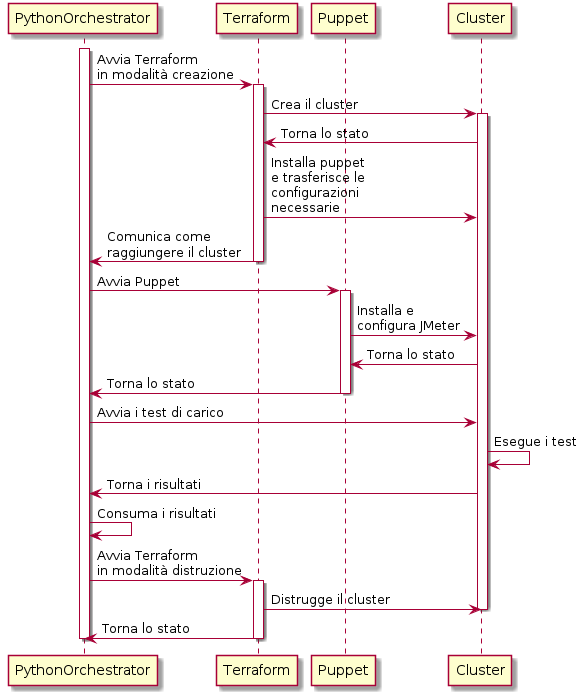
\includegraphics[width=13cm]{immagini/soluzione}
	\caption{Visione ad alto livello della soluzione proposta}
	\label{img-soluzione}
\end{figure}
